\chapter{Evaluierung}

\anno{ca. 10 Seiten} %Ref. hat 5

\section{Aufbau der Testumgebung}
% Aufbau der Messumgebung (1-2 Seiten)

\begin{figure}[bht]
  \begin{center}
    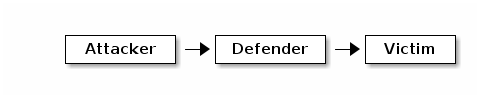
\includegraphics[width=10cm]{pattern}
    \caption{Muster für Tests}
    \label{fig.pattern}
  \end{center}
\end{figure}

\begin{table}[bht]
    \centering
    \begin{tabular}{ |c|c|c|c| } 
      \hline
    Testlauf & Angreifer & Verteidiger & Opfer \\ 
     \hline
     1 & manuell & - & PF showcase\\
     2 & manuell & WebCastellum & PF showcase \\
     3 & ZAP (passiv) & - & PF showcase\\
     4 & ZAP (passiv) & WebCastellum & PF showcase \\
     5 & ZAP (aktiv) & - & PF showcase\\
     6 & ZAP (aktiv) & WebCastellum & PF showcase \\
     7 & manuell & - & WebGoat \\ 
    8 & manuell & WebCastellum & WebGoat \\
    9 & ZAP (passiv) & - & WebGoat \\ 
    10 & ZAP (passiv) & WebCastellum & WebGoat \\
    11 & ZAP (aktiv) & - & WebGoat \\ 
    12 & ZAP (aktiv) & WebCastellum & WebGoat \\
   \hline
    \end{tabular}
    \caption{Testplan}
    \label{tab:testplan}
\end{table}

% Ergebnisse und Beobachtungen (3-4 Seiten)
\section{Ergebnisse und Beobachtungen}

\anno{Tabellenwert!}

%lohnt es sich Training mit altem und neuen Datensatz zu testen? Zeit?

\begin{table}[bht]
    \centering
    \begin{tabular}{ |c|c|c|c|c|c| } 
      \hline
    Testlauf & Angreifer & Verteidiger & Opfer & Schwachstellen & Verbesserung(in \%) \\ 
     \hline
     1 & manuell & - & PF showcase & 3 &\\
     2 & manuell & WebCastellum & PF showcase & 1 & 66\\
     3 & ZAP (passiv) & - & PF showcase & 16 &\\
     4 & ZAP (passiv) & WebCastellum & PF showcase & 2 & 87.5 \\
     5 & ZAP (aktiv) & - & PF showcase & 56 & \\
     6 & ZAP (aktiv) & WebCastellum & PF showcase & 20 & 64.3\\
     7 & manuell & - & WebGoat & 10 & \\ 
    8 & manuell & WebCastellum & WebGoat & 3 & 70 \\
    9 & ZAP (passiv) & - & WebGoat & 25 & \\ 
    10 & ZAP (passiv) & WebCastellum & WebGoat & 12 & 50\\
    11 & ZAP (aktiv) & - & WebGoat & 34 & \\ 
    12 & ZAP (aktiv) & WebCastellum & WebGoat & 14 & 59 \\
   \hline
    \end{tabular}
    \caption{Ergebnisse}
    \label{tab:tes1tergebnisse}
\end{table}


% Diskussion und Bewertung (3-4 Seiten)
\section{Bewertung}


% Zusammenfassung: ca. 0,5 Seiten


\section{Zusammenfassung}
